\documentclass[class=report, crop=false]{standalone}
\usepackage[subpreambles=true]{standalone}
\usepackage{float}

\begin{document}
    \section{Sektionering}
    VI kan lige tage et kig på hierarkiet for sektioner.
    \begin{figure}[H]
        \centering
            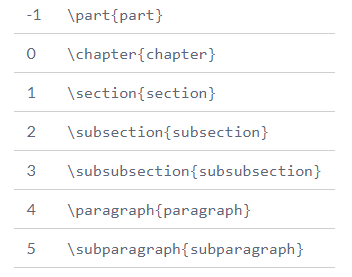
\includegraphics{Sectioning.png}
            \caption{Hierarki over sektioner i \LaTeX.}
            \label{fig:Hierarki}
    \end{figure}
    \noindent Vi laver nu 2 under sektioner for at illustrerer hvordan en sektioner kan være nummereret eller ikke nummereret.

    \subsection{Nummereret sektion}
    Dette er en nummereret sektion og den laves på følgende måde:
    \begin{tcolorbox}
        \verb|\subsection{Nummereret sektion}|
    \end{tcolorbox}

    \subsection*{Ikke nummereret sektion}
    \label{IkkeNummereret}
    \addcontentsline{toc}{section}{2.6.2 \nameref{IkkeNummereret}}
    Dette er en \underline{ikke} nummereret sektion og den laves på følgende måde:
    \begin{tcolorbox}
        \verb|\subsection*{Ikke nummereret sektion}|
    \end{tcolorbox}
    \noindent Bemærk at der dog ikke automatisk bliver angivet en reference til en ikke nummereret sektion og derfor har vi brug for følgende linje i sektionene hvis vi ønsker den skal med i indholdsfortegnelsen:
    \begin{tcolorbox}
        \verb|\subsection*{Ikke nummereret sektion}|\\
        \verb|\label{IkkeNummereret}|\\
        \verb|\addcontentsline{toc}{section}{2.6.2 \nameref{IkkeNummereret}}|
    \end{tcolorbox}
    \noindent Som det fremgår i indholdsfortegnelsen bliver dette noget rod så vælg enten den ene eller anden løsning.
\end{document}